\documentclass{beamer}
\usetheme{Madrid}
\usepackage{amsmath, amssymb}
\usepackage{siunitx}
\sisetup{per-mode=symbol}

\usepackage{tikz}
\usetikzlibrary{arrows.meta, positioning}

\title[Hall Thrusters]{Operating Principles of Hall Effect Thrusters}
\author{Your Name}
\institute{Electric Propulsion Overview}
\date{\today}

\begin{document}

%------------------------------------------------
\begin{frame}
  \titlepage
\end{frame}
%------------------------------------------------

\begin{frame}{What is a Hall Effect Thruster?}
  \begin{itemize}
    \item A Hall Effect Thruster (HET) accelerates ions electrostatically 
          using a crossed electric and magnetic field geometry.
    \item Key feature: \textbf{electrons are magnetized, ions are not}.
    \item Electrons undergo an azimuthal $\mathbf{E}\times\mathbf{B}$ Hall drift.
    \item Unmagnetized ions are accelerated axially by the electric field 
          and exit at $\sim\!10$--$20~\mathrm{km/s}$.
    \item Quasi-neutral plasma throughout; no grids.
  \end{itemize}
\end{frame}
%------------------------------------------------

\begin{frame}{Hall Thruster Geometry (Annular Channel)}
  \begin{columns}
    \begin{column}{0.55\textwidth}
      \begin{itemize}
        \item Ceramic discharge channel with:
          \begin{itemize}
            \item Radial magnetic field $B_r$
            \item Axial electric field $E_z$
            \item Neutral gas injection near anode
            \item Cathode external to the channel
          \end{itemize}
        \item Crossed-field configuration traps electrons,
              enabling efficient ionization and acceleration.
      \end{itemize}
    \end{column}
    \begin{column}{0.45\textwidth}
      \begin{center}
        \textit{(See next slide for TikZ schematic.)}
      \end{center}
    \end{column}
  \end{columns}
\end{frame}
%------------------------------------------------

\begin{frame}{TikZ Schematic: Hall Thruster Cross-Section}
  \centering
  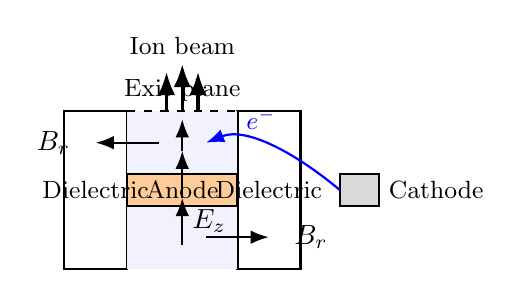
\begin{tikzpicture}[>=Latex, scale=1.0]
    % Channel walls (annular cross section as two rectangles)
    \draw[thick] (-1.5,-1.0) rectangle (-0.7,1.0);
    \draw[thick] (0.7,-1.0) rectangle (1.5,1.0);

    % Channel interior
    \fill[blue!5] (-0.7,-1.0) rectangle (0.7,1.0);

    % Anode at back of channel
    \draw[thick, fill=orange!40] (-0.7,0.2) rectangle (0.7,-0.2);
    \node at (0,0) {\small Anode};

    % Exit plane
    \draw[thick, dashed] (-0.7,1.0) -- (0.7,1.0);
    \node[above] at (0,1.0) {\small Exit plane};

    % Axial E-field arrows (z-direction)
    \draw[->, thick] (0,-0.7) -- (0,-0.1) node[midway, right] {$E_z$};
    \draw[->, thick] (0,-0.1) -- (0,0.5);
    \draw[->, thick] (0,0.5) -- (0,0.9);

    % Radial B-field arrows (from inner to outer wall)
    \draw[->, thick] (-0.3,0.6) -- (-1.1,0.6);
    \draw[->, thick] (0.3,-0.6) -- (1.1,-0.6);
    \node[left] at (-1.3,0.6) {$B_r$};
    \node[right] at (1.3,-0.6) {$B_r$};

    % Ion beam arrows
    \draw[->, very thick] (0,1.0) -- (0,1.6);
    \draw[->, very thick] (-0.2,1.0) -- (-0.2,1.5);
    \draw[->, very thick] (0.2,1.0) -- (0.2,1.5);
    \node[above] at (0,1.6) {\small Ion beam};

    % Cathode outside channel
    \draw[thick, fill=gray!30] (2.0,0.2) rectangle (2.5,-0.2);
    \node[right] at (2.5,0.0) {\small Cathode};

    % Electrons from cathode
    \draw[->, thick, blue] (2.0,0.0) .. controls (1.4,0.5) and (0.8,0.8) .. (0.3,0.6);
    \node[blue] at (1.0,0.9) {\small $e^-$};

    % Channel labels
    \node at (-1.1,0) {\small Dielectric};
    \node at (1.1,0) {\small Dielectric};

  \end{tikzpicture}
\end{frame}
%------------------------------------------------

\begin{frame}{Electron and Ion Magnetization}
  \small
  \textbf{Electrons:} strongly magnetized  
  $$
  r_{L,e} = \frac{m_e v_\perp}{e B} \ll \text{channel size}
  $$
  \textbf{Ions:} effectively unmagnetized  
  $$
  r_{L,i} = \frac{m_i v_\perp}{e B} \gg \text{channel size}
  $$
  \begin{itemize}
    \item Electrons are confined laterally by $B_r$, limiting axial motion.
    \item Ions move freely along the electric field.
    \item Magnetized electrons $\rightarrow$ high ionization efficiency.
  \end{itemize}
\end{frame}
%------------------------------------------------

\begin{frame}{$\mathbf{E}\times\mathbf{B}$ Hall Drift (TikZ View)}
  \centering
  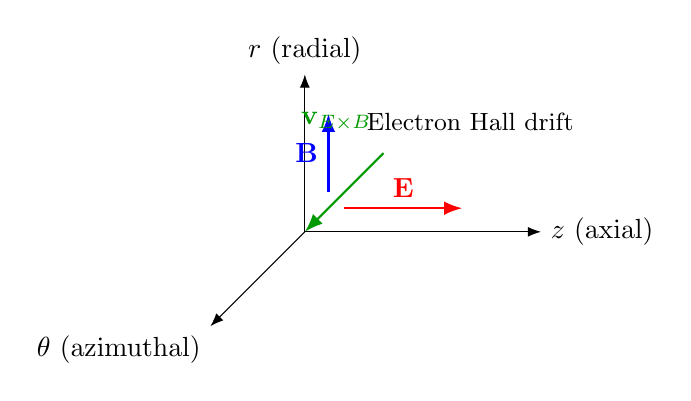
\begin{tikzpicture}[>=Latex, scale=1.0]
    % Coordinate axes
    \draw[->] (0,0) -- (3.0,0) node[right] {$z$ (axial)};
    \draw[->] (0,0) -- (0,2.0) node[above] {$r$ (radial)};
    \draw[->] (0,0) -- (-1.2,-1.2) node[below left] {$\theta$ (azimuthal)};

    % E field along z
    \draw[->, thick, red] (0.5,0.3) -- (2.0,0.3) node[midway, above] {$\mathbf{E}$};

    % B field radial
    \draw[->, thick, blue] (0.3,0.5) -- (0.3,1.5) node[midway, left] {$\mathbf{B}$};

    % v_E x B direction
    \draw[->, thick, green!60!black] (1.0,1.0) -- (0.0,0.0);
    \node[green!60!black] at (0.4,1.4) {$\mathbf{v}_{E\times B}$};

    % Electron drift label
    \node at (2.1,1.4) {\small Electron Hall drift};

  \end{tikzpicture}

  \vspace{0.5em}
  \small
  \begin{itemize}
    \item Crossed fields:
      $$
      \mathbf{v}_{E\times B} = \frac{\mathbf{E}\times\mathbf{B}}{B^2}
      $$
    \item For HET:
      $$
      \mathbf{E} = E_z \hat{z}, \quad \mathbf{B} = B_r \hat{r}
      $$
      $$
      \Rightarrow \mathbf{v}_\theta = \frac{E_z}{B_r} \hat{\theta}
      $$
  \end{itemize}
\end{frame}
%------------------------------------------------

\begin{frame}{$\mathbf{E}\times\mathbf{B}$ Hall Drift}
  \begin{itemize}
    \item Electrons experience crossed electric and magnetic fields:
      $$
      \mathbf{v}_{E\times B} =
      \frac{\mathbf{E}\times\mathbf{B}}{B^2}
      $$
    \item For HET geometry:
      $$
      \mathbf{E} = E_z \hat{z},
      \qquad
      \mathbf{B} = B_r \hat{r}
      $$
      $$
      \Rightarrow\quad
      \mathbf{v}_\theta = \frac{E_z}{B_r} \hat{\theta}
      $$
    \item This azimuthal electron drift current is the \textbf{Hall current}.
    \item Drift enhances electron residence time, boosting ionization.
  \end{itemize}
\end{frame}
%------------------------------------------------

\begin{frame}{Ionization and Acceleration}
  \begin{itemize}
    \item Neutral xenon injected at the anode.
    \item Magnetized electrons drift azimuthally, colliding with neutrals:
      $$
      \mathrm{Xe} + e^- \rightarrow \mathrm{Xe}^+ + 2e^-
      $$
    \item Ionization zone forms near the channel exit.
    \item Ions accelerate axially:
      $$
      F = q E_z, \qquad
      v_i = \sqrt{\frac{2 q V_b}{m_i}}
      $$
    \item Typical ion energies: $200$--$300~\mathrm{eV}$.
  \end{itemize}
\end{frame}
%------------------------------------------------

\begin{frame}{Quasi-Neutral Plasma Acceleration}
  \begin{itemize}
    \item Unlike gridded ion engines (GITs), HETs maintain \textbf{quasi-neutral plasma}
          throughout the acceleration region.
    \item No space-charge-limited extraction:
          electron confinement by $B_r$ limits axial mobility.
    \item Very high ion current densities are achievable ($\sim$ tens of mA/cm$^2$).
    \item The thruster and cathode together produce a \textbf{neutralized ion beam}.
  \end{itemize}
\end{frame}
%------------------------------------------------

\begin{frame}{Cathode Functions}
  \begin{itemize}
    \item Located outside the channel.
    \item Provides electrons for:
      \begin{itemize}
        \item Beam neutralization
        \item Sustaining the discharge current
        \item Replacing electrons lost to the anode
      \end{itemize}
    \item Cathode coupling is essential for efficiency and stability.
  \end{itemize}
\end{frame}
%------------------------------------------------

\begin{frame}{Hall Thrusters vs. Gridded Ion Thrusters (GIT)}
  \small
  \begin{tabular}{p{0.32\textwidth} p{0.30\textwidth} p{0.30\textwidth}}
    \hline
    & \textbf{Hall Effect Thruster} & \textbf{Gridded Ion Thruster} \\
    \hline
    Ion acceleration & Electrostatic, in quasi-neutral plasma; $E_z$ in channel & Electrostatic, through grid apertures; strong sheath and space-charge region \\
    \hline
    Ion optics & No grids; plasma expansion at exit & Multi-grid optics (screen, accel, often decel); tightly controlled beam \\
    \hline
    Electron dynamics & Strongly magnetized; $\mathbf{E}\times\mathbf{B}$ Hall drift & Not strongly magnetized (typically); electrons confined by grids \\
    \hline
    Limiting physics & Cross-field electron transport & Child--Langmuir space-charge limit in grid gaps \\
    \hline
    Thrust-to-power & $\sim 60$--$70~\mathrm{mN/kW}$ & Typically lower, $\sim 30$--$50~\mathrm{mN/kW}$ \\
    \hline
    Efficiency & $\sim 50$--$65\%$ & $\sim 60$--$70\%$ (varies with design) \\
    \hline
    Lifetime limiters & Channel wall erosion, cathode wear & Grid erosion (screen/accelerator), cathode wear \\
    \hline
    Typical use & Orbit raising, station-keeping, all-electric GEO, deep space & Deep space missions, precision pointing, high Isp low thrust \\
    \hline
  \end{tabular}
\end{frame}
%------------------------------------------------

\begin{frame}{Advantages of Hall Thrusters}
  \begin{itemize}
    \item High thrust-to-power ratio ($60$--$70~\mathrm{mN/kW}$).
    \item Efficient: $50$--$65\%$.
    \item Long lifetime with magnetic shielding designs.
    \item Simple, robust design: no grids, tolerant to contamination.
    \item Widely used for Earth-orbit raising, station-keeping, and deep-space missions.
  \end{itemize}
\end{frame}
%------------------------------------------------

\begin{frame}{Summary of HET Operation}
  \begin{itemize}
    \item Crossed $E_z$ and $B_r$ fields trap electrons and cause a strong 
          $\mathbf{E}\times\mathbf{B}$ Hall drift.
    \item Trapped electrons enhance ionization efficiency near the channel exit.
    \item Ions, unmagnetized, are accelerated by the axial electric field.
    \item A cathode provides electrons to neutralize the ion beam.
    \item Result: efficient, stable, quasi-neutral plasma acceleration.
  \end{itemize}
\end{frame}
%------------------------------------------------

\end{document}